Dado el siguiente modelo de Programación Lineal:
\begin{equation}
\begin{split}
\mbox{max. } z = 2x_1 + 1x_2 -5 x_3\\
s.a.:\\
-x_1 -x_2 + x_3 \leq -4\\
x_1 +  x_2 +  x_3 \leq 2\\
x_1,\,x_2,\,x_3 \geq 0
\end{split}
\end{equation}

Obtén su solución óptima resolviendo gráficamente su problema dual.

---

El problema dual es:
\begin{equation}
\begin{split}
\mbox{max. } z = -4y_1+2y_2\\
s.a.:\\
-y_1 + y_2 \geq 2\\
-y_1 + y_2 \geq 1\\
y_1+y_2 \geq -5\\
y_1,\, y_2\geq 0
\end{split}
\end{equation}

\definecolor{zzttqq}{rgb}{0.6,0.2,0}
\definecolor{qqqqff}{rgb}{0,0,1}
\begin{figure}[h]
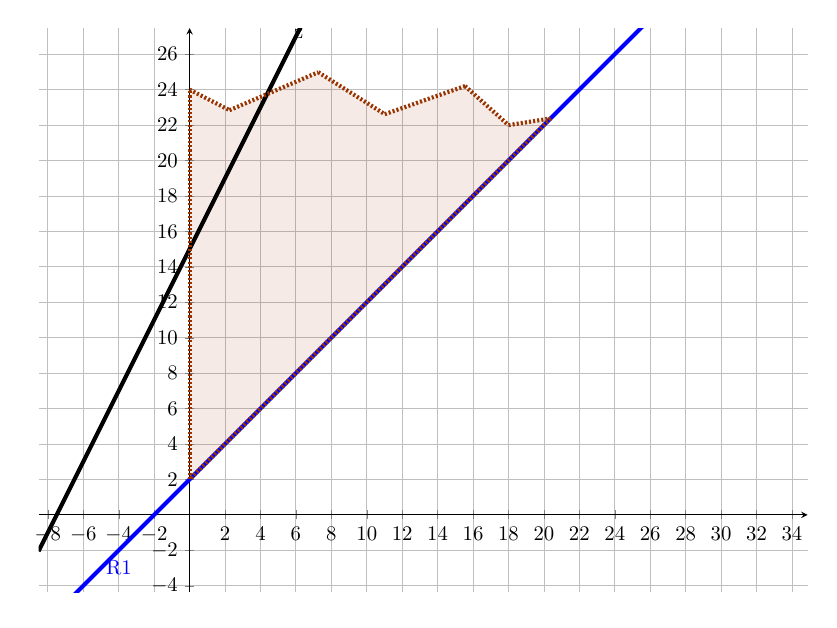
\begin{tikzpicture}[scale = 0.75][line cap=round,line join=round,>=triangle 45,x=0.5cm,y=0.5cm]
\begin{axis}[
x=0.3cm,y=0.3cm,
axis lines=middle,
ymajorgrids=true,
xmajorgrids=true,
xmin=-8.524178618707172,
xmax=34.88658602326376,
ymin=-4.3764822985158744,
ymax=27.476543961399035,
xtick={-8,-6,...,34},
ytick={-4,-2,...,26},]
\clip(-8.524178618707172,-4.3764822985158744) rectangle (34.88658602326376,27.476543961399035);
\fill[line width=2pt,dash pattern=on 1pt off 1pt,color=zzttqq,fill=zzttqq,fill opacity=0.10000000149011612] (0,2) -- (0,24) -- (2.2529717680466326,22.843376505411413) -- (7.263843092728892,24.98369842801439) -- (11.015701521762342,22.616754184194626) -- (15.548147946098055,24.203110432712126) -- (18,22) -- (20.373854535227174,22.373854535227174) -- cycle;
\draw [line width=2pt,domain=-8.524178618707172:34.88658602326376] plot(\x,{(--30--4*\x)/2});
\draw [line width=2pt,color=qqqqff,domain=-8.524178618707172:34.88658602326376] plot(\x,{(--2--1*\x)/1});
\draw [line width=2pt,dash pattern=on 1pt off 1pt,color=zzttqq] (0,2)-- (0,24);
\draw [line width=2pt,dash pattern=on 1pt off 1pt,color=zzttqq] (0,24)-- (2.2529717680466326,22.843376505411413);
\draw [line width=2pt,dash pattern=on 1pt off 1pt,color=zzttqq] (2.2529717680466326,22.843376505411413)-- (7.263843092728892,24.98369842801439);
\draw [line width=2pt,dash pattern=on 1pt off 1pt,color=zzttqq] (7.263843092728892,24.98369842801439)-- (11.015701521762342,22.616754184194626);
\draw [line width=2pt,dash pattern=on 1pt off 1pt,color=zzttqq] (11.015701521762342,22.616754184194626)-- (15.548147946098055,24.203110432712126);
\draw [line width=2pt,dash pattern=on 1pt off 1pt,color=zzttqq] (15.548147946098055,24.203110432712126)-- (18,22);
\draw [line width=2pt,dash pattern=on 1pt off 1pt,color=zzttqq] (18,22)-- (20.373854535227174,22.373854535227174);
\draw [line width=2pt,dash pattern=on 1pt off 1pt,color=zzttqq] (20.373854535227174,22.373854535227174)-- (0,2);
\begin{scriptsize}
\draw[color=black] (6.15591174455794,27.161790737486832) node {z};
\draw[color=qqqqff] (-3.99173219437146,-2.953797726432718) node {R1};
\end{scriptsize}
\end{axis}
\end{tikzpicture}
\end{figure}

El problema dual es factible no acotado. Luego el primal es no factible.